\documentclass[12pt]{article}
\usepackage[pdfborder={0 0 0.5 [3 2]}]{hyperref}%
\usepackage[left=1in,right=1in,top=1in,bottom=1in]{geometry}%
\usepackage[shortalphabetic]{amsrefs}%
\usepackage{amsmath}
\usepackage{enumerate}
\usepackage{enumitem}
\usepackage{amssymb}                
\usepackage{amsmath}                
\usepackage{amsfonts}
\usepackage{amsthm}
\usepackage{bbm}
\usepackage[table,xcdraw]{xcolor}
\usepackage{tikz}
\usepackage{float}
\usepackage{booktabs}
\usepackage{svg}
\usepackage{mathtools}
\usepackage{cool}
\usepackage{url}
\usepackage{graphicx,epsfig}
\usepackage{framed}
\usepackage{hyperref}  

\usetikzlibrary{automata,arrows,positioning,calc}
\DeclarePairedDelimiter\abs{\lvert}{\rvert}%
\DeclarePairedDelimiter\norm{\lVert}{\rVert}%
\DeclarePairedDelimiter\ceil{\lceil}{\rceil}
\DeclarePairedDelimiter\floor{\lfloor}{\rfloor}

\makeatletter
\renewcommand*\env@matrix[1][*\c@MaxMatrixCols c]{%
  \hskip -\arraycolsep
  \let\@ifnextchar\new@ifnextchar
  \array{#1}}
\makeatother

\newtheorem{theorem}{Theorem}[section]
\newtheorem{corollary}{Corollary}[theorem]
\newtheorem{proposition}[theorem]{Proposition}
\newtheorem{lemma}[theorem]{Lemma}

\theoremstyle{definition}
\newtheorem{definition}[theorem]{Definition}
\newtheorem{exercise}{Exercise}%
\newtheorem{problem}[exercise]{Problem}%
\newtheorem*{example}{Example}

\theoremstyle{remark}
\newtheorem*{question}{Question}
\newtheorem*{observation}{Observation}
\newtheorem*{remark}{Remark}

\graphicspath{ {images/} }

\setlength{\parindent}{0cm}
\renewcommand{\vec}[1]{\ensuremath{\mathbf{#1}}}

\def\noi{\noindent}
\def\T{{\mathbb T}}
\def\R{{\mathbb R}}
\def\N{{\mathbb N}}
\def\C{{\mathbb C}}
\def\Z{{\mathbb Z}}
\def\P{{\mathbb P}}
\def\E{{\mathbb E}}
\def\Q{\mathbb{Q}}
\def\ind{{\mathbb I}}

\def\cale{{\mathcal E}}
\def\cals{{\mathcal S}}
\def\calc{{\mathcal C}}
\def\caln{{\mathcal N}}
\def\calb{{\mathcal B}}
\def\calg{{\cal G}}

\def\ds{\displaystyle}
\def\ra{\rightarrow}
\newcommand{\conv}{\mbox{\rm conv}}
\newcommand{\spaan}{\mbox{\rm span}}
\newcommand{\deet}{\mbox{\rm det}}
\newcommand{\aff}{\mbox{\rm aff}}
\newcommand{\cl}{\mbox{\rm cl}}
\newcommand{\dimm}{\mbox{\rm dim}}
\newcommand{\sm}{\setminus}
\def\ci{\perp\!\!\!\perp}

\newcommand{\ink}{\rule{.5\baselineskip}{.55\baselineskip}}

\begin{document}

\setcounter{section}{4}
\section{Sampling Distributions}

\subsection{Introduction}

In this section, we transition from the world of probability to the world of statistics. The field of probability is concerned with making predictions about probability distributions which are completely known. The contents of a deck of cards, for example, is known, and thus we can derive probabilistic statements about the likelihood of certain cards being flipped in a game of Texas Hold'em poker. The field of statistics addresses the converse problem. It allows us to make inferences about the distribution of a population based on a small sample drawn from that population. We then use the tools from probability to make probabilistic statements about the accuracy of our inferences. For example, we can model the distribution of Rhode Island voter preferences in the gubernatorial election with a binomial distribution. The parameters of the distribution are $n = 754,224$ (the number of registered voters as of election day, 2014) and $p$, the proportion of voters who prefer Gina Raimondo. The parameter $p$ is unknown, and unless we accurately survey every single registered voter, we will not know its exact value. Such a survey is logistically and financially unfeasible, thus we turn to statistics. We poll a smaller sample of voters (say, 1000) and find the proportion of voters in that smaller sample who prefer Raimondo. This sample proportion is designated $\hat{p}$, where the ``hat'' indicates that it is an estimator for the true value $p$ based off of a sample drawn from the larger population. Using the tools of statistics, we will be able to quantitatively evaluate how close our estimate $\hat{p}$ is to the true value $p$.\\

\subsection{Statistics}

We will use the following setup for our discussion.
\begin{enumerate}
\item We have a large population and are interested in studying a particular quantitative feature of that population. For example, the population could be the registered voters in Rhode Island, and we are interested in the yes/no question ``Are you going to vote for Raimondo?''. Another population could be the ball bearings produced by the factory, and we are interested in their diameter.
\item The population feature can be characterized by a pmf $p(y)$ (if it is discrete, as in the case of the number of voters who prefer Raimondo) or a density function $f(y)$ (if it is continuous, as in the case of the ball bearing diameters).
\item The population feature will have certain parameters. All populations have a mean and a variance, which will be designated by $\mu$ and $\sigma^2$. We will refer to these as the population mean and the population variance. Populations may also have other parameters. As an example, if we model a population with a uniform distribution on an unknown interval $[a, b]$, the endpoints $a$ and $b$ are parameters of the population. Much of statistics is concerned with estimating parameters of populations.
\item We take a small sample from the population. Let $n$ be the sample size, and let the random variables $Y_1, \dots, Y_n$ be the samples we take from the population. 
\item We will assume that the sample size is small enough relative to the population size that the samples $Y_1, \dots, Y_n$ are independent and have the same distribution $p(y)$ or $f(y)$ as the population. As an example, recall that we mentioned before that sampling without replacement (as in political polling) was approximately binomial if the sample size was less than 1/20 of the population size.
\item A \emph{statistic} is a function of our samples $Y_1, \dots, Y_n$. The function can only involve the samples themselves and known constants such as the sample size $n$. Since a statistic is a function of random variables, it is itself a random variable, thus we can characterize its distribution using the tools of probability. 
\end{enumerate}
In this first section we will be concerned with the probability distribution of various statistics. Before we continue, we will give a table of the most common statistics we will encounter. Let $Y_1, \dots, Y_n$ be independent and identically distributed (iid) samples drawn from a population which is distributed according to a pmf $p(y)$ or a density $f(y)$. Let $\mu$ and $\sigma^2$ be the population mean and variance.

\begin{figure}[H]
\centering
\label{my-label}
\begin{tabular}{@{}ll@{}}
\toprule
Statistic                                 & Definition                                           \\ \midrule
sample mean                               & $\bar{Y} = \frac{1}{n} \sum_{i=1}^n Y_i$             \\
sample variance                           & $S^2 = \frac{1}{n-1} \sum_{i=1}^n (Y_i - \bar{Y})^2$ \\
smallest order statistic (sample minimum) & $Y_{1} = \min(Y_1, \dots, Y_n)$                      \\
largest order statistic (sample maximum)  & $Y_{n} = \max(Y_1, \dots, Y_n)$                      \\
sample range                              & $R = Y_{n} - Y_{1}$                                  \\ \bottomrule
\end{tabular}
\end{figure}

Note that you have to compute $\bar{Y}$ before you can compute $S^2$. The $n-1$ in the denominator of the sample variance may seem a bit mysterious, but we will see in a few classes why that makes sense. For now, we will look at the sample mean. To get the sample mean, we add together the samples and divide by the number of samples, so this is the empirical mean we have discussed before. The sample mean is a random variable, so we can find its mean and variance. Using linearity of expectation and the fact that all the $Y_i$ have expected value of $\mu$,
\begin{align*}
\E(\bar{Y}) &= \E\left(\frac{1}{n} \sum_{i=1}^n Y_i\right)\\
&= \frac{1}{n} \sum_{i=1}^n \E(Y_i)\\
&= \frac{1}{n} \sum_{i=1}^n \mu \\
&= \frac{1}{n} n \mu \\
&= \mu
\end{align*}
Thus the expected value of the sample mean is the population mean $\mu$.\\

For the variance, we recall that $Var(aY) = a^2 Var(Y)$ and that for independent random variables, $Var(Y_1 + \cdots + Y_n) = Var(Y_1) + \cdots + Var(Y_n)$. Using this plus the fact the all the $Y_i$ have variance of $\sigma^2$,
\begin{align*}
Var(\bar{Y}) &= Var\left(\frac{1}{n} \sum_{i=1}^n Y_i\right)\\
&= \frac{1}{n^2} \sum_{i=1}^n Var(Y_i)\\
&= \frac{1}{n^2} \sum_{i=1}^n \sigma^2 \\
&= \frac{1}{n^2} n \sigma^2 \\
&= \frac{\sigma^2}{n}
\end{align*}
The variance of the sample mean is thus the population variance divided by $n$. As $n$ gets larger, this variance gets smaller, which makes intuitive sense since there should be less spread if we average more samples together.\\

Note that while we have characterized the mean and variance of the sample mean, we have said nothing about its distribution. In general, there is not much additional we can say. In the special case where the population has a normal distribution, however, we can say a lot more.

\subsection{Sampling Distributions for Normally Distributed Populations}

\subsubsection{Distribution of Sample Mean}

Suppose we have a population which is normally distributed. Then the sample mean is also normally distributed.

\begin{framed}
Let $Y_1, \dots, Y_n$ be a sample of size $n$ drawn from a population which has a normal distribution with mean $\mu$ and variance $\sigma^2$. Then the sample mean
\[
\bar{Y} = \frac{1}{n} \sum_{i=1}^n Y_i
\]
has a normal distribution with mean $\E(\bar{Y}) = \mu$ and variance $Var(\bar{Y}) = \sigma^2 / n$.
\end{framed}
The mean and variance of the sample mean was shown above. To show the sample mean has a normal distribution, we can use the method of moment generating functions or characteristic functions, which will not be done in this course for sake of time.\\

Since the sample mean $\bar{Y}$ is normally distributed with mean $\mu$ and variance $\sigma^2 / n$, 
\[
Z = \frac{\bar{Y} - \mu}{\sigma / \sqrt{n} } = \sqrt{n}\left( \frac{\bar{Y} - \mu}{\sigma }\right)
\]
is a standard normal random variable. (Recall that to get a standard normal, we subtract the mean and divide by the standard deviation, which is the square root of the variance.)\\

Let's use this in an example.

\begin{example}A ball bearing machine produces ball bearings whose diameters are normally distributed with mean $
\mu$ mm and standard deviation $\sigma$ mm. We unfortunately have lost the manual for the machine, so we do not know the value of $\mu$. We call the company to get more information, but all they can tell us is that $\sigma = 0.1$. 

\begin{enumerate}
\item We take a sample of 16 ball bearings from the machine and compute the sample mean $\bar{Y}$. Find the probability that $\bar{Y}$ is within 0.02 mm of the true mean $\mu$.\\


By what we learned above, the sample mean $\bar{Y}$ has a normal distribution with mean $\mu$ and variance $\sigma^2 / n = 0.1^2 / 16$. The standard deviation of $\bar{Y}$ is $\sigma = 0.1 / \sqrt{16}$. Thus we can find the probability by converting to the standard normal distribution.

\begin{align*}
\P( |\bar{Y} - \mu| \leq 0.02) &= \P( -0.02 \leq (\bar{Y} - \mu) \leq 0.02 ) \\
&= \P\left( \frac{-0.02}{\sigma/\sqrt{n}} \leq \frac{\bar{Y} - \mu}{\sigma/\sqrt{n}} \leq \frac{0.02}{\sigma/\sqrt{n}}  \right) \\
&= \P\left( \frac{-0.02}{0.1/\sqrt{16}} \leq Z \leq \frac{0.02}{0.1/\sqrt{16}} \right)\\
&= \P(-0.8 \leq Z \leq 0.8) \\
&= 0.7881 - 0.2119\\
&= 0.5762
\end{align*}

\item How many ball bearings should we sample if we wish the sample mean to be within 0.02 mm of $\mu$ with probability 0.95?\\

We can use the 68-95-99.7 rule here. We want the sample mean to be with 0.02 mm of the mean with probability 0.95. Another way of writing this is that we want the population mean $\mu$ to lie within two sample standard deviations of the sample mean. Thus we want the sample standard deviation to be $0.02 / 2 = 0.01$. Since the sample standard deviation is $\sigma / \sqrt{n} = 0.1 / \sqrt{n}$, all we have to is set these equal to each other and solve for $n$.
\begin{align*}
\frac{0.1}{\sqrt{n}} &= 0.01 \\
\sqrt{n} &= \frac{0.1}{0.01} = 10 \\
n &= 100
\end{align*} 

\item How many ball bearings should we sample if we wish the sample mean to be within 0.02 mm of $\mu$ with probability 0.99?\\

Here we can't rely on the 68-95-99.7 rule and have to actually do the math. We want:
\begin{align*}
\P( |\bar{Y} - \mu| \leq 0.02) &= \P( -0.02 \leq (\bar{Y} - \mu) \leq 0.02 ) = 0.99
\end{align*}
Dividing this by the sample standard deviation $\sigma / \sqrt{n}$ to convert to the standard normal, we get
\begin{align*}
0.99 &= \P\left( \frac{-0.02}{\sigma/\sqrt{n}} \leq \frac{\bar{Y} - \mu}{\sigma/\sqrt{n}} \leq \frac{0.02}{\sigma/\sqrt{n}}  \right) \\
&= \P\left( \frac{-0.02}{0.1/\sqrt{n}} \leq Z \leq \frac{0.02}{0.1/\sqrt{n}} \right)\\
&= \P(-0.2 \sqrt{n} \leq Z \leq 0.2 \sqrt{n}) \\
\end{align*}
At this point, we take complements and use the symmetry of the normal distribution.
\begin{align*}
\P(Z \leq -0.2 \sqrt{n} \text{ or } Z \geq 0.2 \sqrt{n}) &= 1 - 0.99 = 0.01 \\
\P(Z \leq -0.2 \sqrt{n}) = 0.005
\end{align*}
Consulting a $Z$ table, we find that $\P(Z \leq -2.57) = 0.0051$ and $\P(Z \leq -2.58) = 0.0049$. Choosing the first one (you can choose either one) and setting that value of $z$ equal to $-0.2 \sqrt{n}$, we get:
\begin{align*}
-0.2 \sqrt{n} &= -2.57 \\
\sqrt{n} &= 12.85 \\
n &= 165.123
\end{align*}
Rounding up to the nearest integer, we need a sample size of 166 or more to have 99\% confidence that our sample mean is within 0.02 of the true population mean.
\end{enumerate}

\end{example}

\subsection{Other distributions}
We will now briefly discuss two other useful distributions, the chi-square and $t$ distribution. Since computations with these distributions is done via tables and not by using the densities directly, we will not give the densities here. If you are curious what these densities look like, you can consult Wikipedia or a statistics textbook.\\

\subsubsection{Chi-square distribution}

\emph{This section was not covered in class but is included for completeness; unless I cover it in the future, I am presenting this purely for reference. It will not appear on any problem set or exam.} \\

The chi-square distribution is the distribution of the sum of the squares of independent, standard normal random variables. Since the variance of a random variable is computed by first finding the expected value of the square of the random variable, the chi-square distribution is used when we make inferences about the variance of a population. 

\begin{framed}
Let $Y_1, \dots, Y_n$ be a sample of size $n$ drawn from a population which has a normal distribution with mean $\mu$ and variance $\sigma^2$. Then the random variables $Z_i = (Y_i - \mu)/\sigma$ are independent, standard normal random variables, and
\[
\sum_{i=1}^n Z_i^2 = \sum_{i=1}^n \left( \frac{Y_i - \mu}{\sigma}\right)^2
\]
has a $\chi^2$ (chi-square) distribution with $n$ degrees of freedom (df).
\end{framed}

To use the chi-square distribution, we use a chi-square table, which is provided on the course website. Chi-square tables are a little weird. Here's how we use them. Suppose $Y$ has a chi-square distribution with 10 df. We will be looking at the row labeled 10 df. Now look across the top row. You see $\chi^2_{.995}, \chi^2_{.990}, \chi^2_{.975}$, etc. The decimals there are probabilities. What do they represent? Let's look at the row for 10 df. The first entry in that row, in the column labeled $\chi^2_{.995}$, is the value of $y$ for which $\P(Y > y) = 0.995$. The entry in that box is 2.156, so $\P(Y > 2.156) = 0.995$. If we want the probability that $Y$ is less than or equal to 2.156, then we just subtract from 1 to get $\P(Y \leq 2.156) = 1 - 0.995 = 0.005$. Similarly, looking at the 6th column, we have $\P(Y > 15.987) = 0.100$, so $\P(Y \leq 15.987) = 1 - 0.100 = 0.90$. Note that the probabilities across the top are ``extreme'' probabilities, i.e. very high or very low. In general, those are the probabilities we will be interested in. For other values, you can use a statistical package such as R.\\

First, let's practice using the chi-square table, then we will use the chi-square distribution in an example.

\begin{example}Let $Z_1, \dots, Z_6$ be independent samples from a standard normal distribution. Find a value $a$ such that
\[
\P\left( \sum_{i=1}^6 Z_i^2 \leq a \right) = 0.95
\]
By the above, $\sum_{i=1}^6 Z_i^2$ has a chi-square distribution with 6 df. We want the probability that this is less than $a$ to be 0.95, which is equivalent to 
\[
\P\left( \sum_{i=1}^6 Z_i^2 > a \right) = 1 - 0.95 = 0.05
\]
Thus we look at the chi-square table in the 6 df row and find the entry in the column labeled $\chi^2_{.050}$ to get 12.592. Thus we conclude that $a = 12.592$.
\end{example}

How do we use this practically. Recall from above that the sample variance is given by:
\[
S^2 = \frac{1}{n-1} \sum_{i=1}^n (Y_i - \bar{Y})^2
\]

Then we can say the following about the distribution of $S^2$:
\begin{framed}
Let $Y_1, \dots, Y_n$ be a sample of size $n$ drawn from a population which has a normal distribution with mean $\mu$ and variance $\sigma^2$. Let $S^2$ be the sample variance as given above. Then
\[
\frac{(n-1)S^2}{\sigma^2} = \frac{1}{\sigma^2}\sum_{i=1}^n (Y_i - \bar{Y})^2
\]
has a $\chi^2$ (chi-square) distribution with $n-1$ degrees of freedom (df).
\end{framed}
Again, the proof of this is omitted for sake of time. Let's go back to our ball bearing example.

\begin{example}A ball bearing machine produces ball bearings whose diameters are normally distributed with mean $
\mu$ mm and standard deviation $\sigma$ mm. Once again, all we know is that $\sigma = 0.1$. Suppose we select 10 samples and compute the sample variance $S^2$. Find an interval $[a, b]$ such that the probability that $S^2$ lies in the interval is 0.90, i.e.
\[
\P(a \leq S^2 \leq b) = 0.90
\]
Multiplying by $(n - 1)$ and dividing by $\sigma^2$, we get:
\[
0.90 = \P(a \leq S^2 \leq b) = \P \left( \frac{(n-1)a}{\sigma^2} \leq \frac{(n-1)S^2}{\sigma^2} \leq \frac{(n-1)b}{\sigma^2} \right)
\]
\end{example}
From above, we know that $\frac{(n-1)S^2}{\sigma^2}$ has a chi-square distribution with $(n - 1) = 10 - 1 = 9$ df. Let's call this $X$. Then we have:
\[
0.90 = \P(a \leq S^2 \leq b) = \P \left( \frac{(n-1)a}{\sigma^2} \leq X \leq \frac{(n-1)b}{\sigma^2} \right)
\]
where $X$ has a chi-square distribution with 9 df. There are many ways we can choose $a$ and $b$ to make this happen, but the easiest way is to ``split the difference''. Taking complements, we can write this as:
\[
\P \left( X \leq \frac{(n-1)a}{\sigma^2} \text{ or } X \geq \frac{(n-1)b}{\sigma^2} \right) = 1 - 0.90 = 0.10
\]
Splitting the probability of 0.10 in half, we will find $a$ and $b$ such that:
\[
\P \left( X \leq \frac{(n-1)a}{\sigma^2} \right) = 0.05 \text{ and } \P \left( X \geq \frac{(n-1)b}{\sigma^2} \right) = 0.05
\]
Since the chi-square table gives us probabilities of being greater than a value, this is equivalent to:
\[
\P \left( X > \frac{(n-1)a}{\sigma^2} \right) = 0.95 \text{ and } \P \left( X > \frac{(n-1)b}{\sigma^2} \right) = 0.05
\]
(these are continuous random variables, so the strictness of the inequalities does not matter). Now we look at the chi-square table. We need the values for 0.95 and 0.05 in the 9 df row, which are 3.325 and 16.919. Then we can solve for $a$ and $b$, since we know $n = 10$ and $\sigma = 0.1$.
\begin{align*}
3.325 &= \frac{(n-1)a}{\sigma^2} = \frac{9a}{0.1^2} \\
a &= \frac{3.325 \cdot 0.1^2}{9} = 0.0037
\end{align*}

\begin{align*}
16.919 &= \frac{(n-1)b}{\sigma^2} = \frac{9b}{0.1^2} \\
a &= \frac{16.919 \cdot 0.1^2}{9} = 0.0187
\end{align*}
Thus our interval $[a, b]$ is [0.0037, 0.0187], which has 90\% probability of including our sample variance $S^2$. Note that the true population variance $\sigma^2 = 0.1^2 = 0.01$ lies in that interval. If our sample variance is not in that interval, perhaps we should be suspicious of either our sampling technique or that something is going wrong with the machine.\\

\subsubsection{t distribution}
What happens when we do not know the population standard deviation. Recall that if we have normal population whose mean and standard deviation is known, the quantity
\[
\sqrt{n}\left( \frac{\bar{Y} - \mu}{\sigma }\right)
\] 
is a standard normal random variable (essentially a normalized version of the sample mean). If the population standard deviation is not known, then we can replace $\sigma$ by our sample statistic $S$ (the square root of the population variance $S^2$) to get
\[
\sqrt{n}\left( \frac{\bar{Y} - \mu}{ S }\right)
\]
The probability distribution of this quantity is known as the t-distribution.
\begin{framed}
Let $Y_1, \dots, Y_n$ be a sample of size $n$ drawn from a population which has a normal distribution with mean $\mu$ and unknown variance. Let $S^2$ be the sample variance as given above. Then
\[
T = \sqrt{n}\left( \frac{\bar{Y} - \mu}{ S }\right)
\]
has a t-distribution with $n-1$ degrees of freedom (df).
\end{framed}
The $t$ distribution, like the standard normal $Z$ distribution, is bell-shaped, has a mean of 0, and is symmetric about its mean. However, it has thicker tails than the $Z$ distribution, so outlier values are more common. The following plot shows the standard normal distribution in blue and the t distribution with 4 df in red.

\begin{figure}[H]
\centering
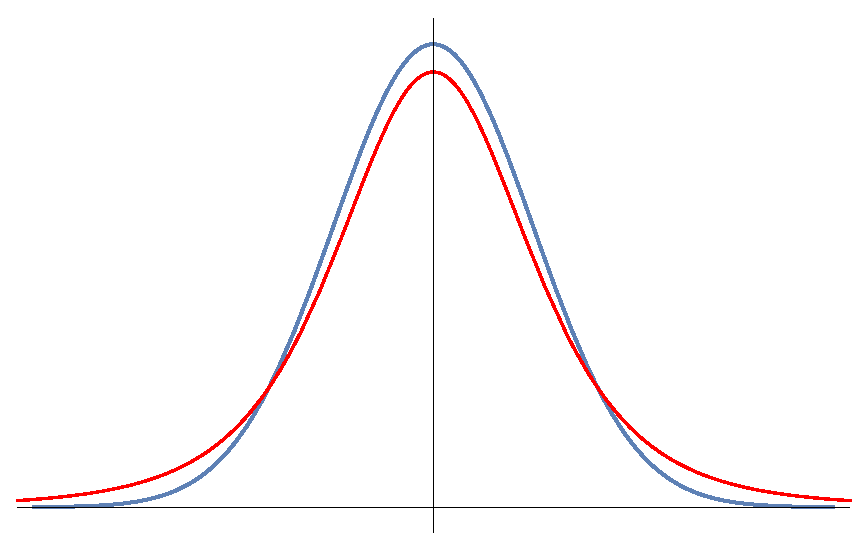
\includegraphics[width=8cm]{tvsz.eps}
\end{figure}

As the number of df gets larger (i.e. approaches infinity), the t distribution approaches the standard normal distribution. Like the Z distribution and chi-square distribution, we use tables to work with the t-distribution. Let's do an example of this. 

\begin{example}Once again, we have a bearing machine produces ball bearings whose diameters are normally distributed with mean $
\mu$ mm and standard deviation $\sigma$ mm. We not only have lost the manual for the machine, but the company has gone bankrupt so they cannot tell us anything about the machine. We take a sample of 16 ball bearings from the machine and compute the sample mean $\bar{Y}$. We also compute the sample standard deviation $S$ and find that $S = 0.1$. Find a range $[a, b]$ such that the probability that the difference between the sample mean and the population mean $\mu$ falls within the interval with a probability of 0.90.\\

We are interested in finding $a$ and $b$ such that $\P(a \leq (\bar{Y} - \mu) \leq b) = 0.90$. Multiplying by $\sqrt{n}$ and dividing by $S$, we get:
\begin{align*}
\P\left( \frac{\sqrt{n}a}{S} \leq \sqrt{n} \left(\frac{\bar{Y} - \mu}{ S }\right) \leq \frac{\sqrt{n}a}{S} \right) &= 0.90\\
\P\left( \frac{\sqrt{16}a}{0.1} \leq T \leq \frac{\sqrt{16}a}{0.1} \right) &= 0.90 \\
\P\left( 40a \leq T \leq 40b  \right) &= 0.90 
\end{align*}
Now we look at our t-table. Note that the t-table gives probabilities for the upper tail of the t-distribution and that the t-distribution is symmetric about the mean. We have a sample of 16, so we want 15 df. We will take a symmetric interval about the mean, so we want $\P(T \leq 40a) = 0.05$ and $\P(T \leq 40b) = 0.05$. For the upper tail, we look at the t-table in the row for 15 df and go across until we get to 0.05, which gives us a t-value of 1.753. By symmetry, the lower t-value is -1.753. Thus we have $40b = 1.753$, which implies $b = 0.0438$. By symmetry, $a = -0.0438$. Thus we are 90\% confident that the difference between the sample and population means falls within the interval $[-0.0438, 0.0438]$.\\

What if we actually know the population standard deviation, as in the example above. Then we can use the standard normal distribution instead of the t-distribution. How does the interval we get compare to that where the population standard deviation is not known. We expect to get a narrower interval in this case, since we have more information. Let's see if that is indeed the case. 
\begin{align*}
\P\left( \frac{\sqrt{n}a}{\sigma} \leq \sqrt{n} \left(\frac{\bar{Y} - \mu}{ \sigma }\right) \leq \frac{\sqrt{n}a}{\sigma} \right) &= 0.90\\
\P\left( \frac{\sqrt{16}a}{0.1} \leq Z \leq \frac{\sqrt{16}a}{0.1} \right) &= 0.90 \\
\P\left( 40a \leq Z \leq 40b  \right) &= 0.90 
\end{align*}
So far, this is exactly the same except we have $Z$ in place of $T$. Again, we will look for a symmetric interval about the mean, so we want $\P(Z \leq 40a) = 0.05$ and $\P(Z \leq 40b) = 0.05$. For the lower tail, we look at the Z-table and can choose either $z = -1.65$ (corresponding to a probability of 0.0495) or $z = -1.64$ (corresponding to a probability of 0.0505). Choosing $z = -1.64$ we get $40a = -1.64$, so $a = -0.041$. By symmetry, $b = 0.041$. Thus we are 90\% confident that the difference between the sample and population means falls within the interval $[-0.041, 0.041]$. As predicted, this is a narrower interval than the case where we used the t-distribution (where the population standard deviation was unknown).
\end{example}

\subsection{Central Limit Theorem}

Take $n$ independent samples $Y_1, \dots, Y_n$ from a population with population mean $\mu$ and population variance $\sigma^2$. Then we showed earlier that the sample mean $\bar{Y} = \frac{1}{n}\sum_{i=1}^n Y_i$ has mean $\E(\bar{Y}) = \mu$ and variance $Var(\bar{Y}) = \sigma^2 / n$. In the case where the population is normally distributed, then $\bar{Y}$ is also normally distributed, i.e. $\bar{Y} \sim$ Normal$(\mu, \sigma/\sqrt{n})$. \\

What is the distribution of $\bar{Y}$ if the population distribution is not normal? It turns out that as long as the sample size is large ($n \geq 30$ is often used as a guideline for ``large''), the sample mean $\bar{Y}$ can be approximated by a normal distribution. This remarkable result is known as the \emph{central limit theorem}.

\begin{framed}
\emph{Central Limit Theorem}\\
  \rule{\dimexpr\linewidth-2\fboxsep-2\fboxrule}{.1pt} \\
Let $Y_1, \dots, Y_n$ be independent and identically distributed (iid) random variables with $\E(Y_i) = \mu$ and $Var(Y_i) = \sigma^2$. Let $\bar{Y}$ be the sample mean, i.e.
\[
\bar{Y} = \frac{1}{n}\sum_{i=1}^n Y_i
\]
Define $U_n$ by
\[
U_n = \frac{\bar{Y} - \mu}{\sigma/\sqrt{n}}
\]
$U_n$ is a normalized version of the sample mean $\bar{Y}$, which we obtain by subtracting the mean and dividing by the standard deviation. Then the distribution of $U_n$ converges to that of a standard normal distribution as $n \rightarrow \infty$. Mathematically, this means that the CDF of $U_n$ converges to the standard normal CDF, i.e.
\[
\lim_{n\rightarrow\infty} \P(U_n \leq u) = \int_{-\infty}^u \frac{1}{\sqrt{2\pi}}e^{-t^2/2} dt
\]
Practically, the means that for a large sample size (approx $n \geq 30$), the sample mean $\bar{Y}$ is asymptotically normally distributed with mean $\mu$ and variance $\sigma^2 / n$.
\end{framed}
The proof of the central limit theorem is complicated and will be omitted for the sake of time. It involves the use of either moment generating functions or characteristic functions and some clever approximations.\\

Let's do some examples.

\begin{example}
Suppose standardized test scores historically have a mean of 60 and variance of 64. New versions are created for every administration of the test. A new version of the test is given to 100 students, and the mean score of those 100 students is 58. How likely is it that there is something wrong with new version of the test.\\

We will compute the probability that the sample mean is less than or equal to 58. Let $\bar{Y}$ be the mean of the sample of 100 students who take the new version. By the central limit theorem, since our sample size is large ($\geq 30$), the sample mean is an approximately normal random variable with mean $\mu = 60$ and variance $\sigma^2 / n = 64 / 100$. The standard deviation of the sample mean is the square root of the variance, i.e. $8/10 = 0.8$. Converting to the standard normal random variable:
\[
\P(\bar{Y} \leq 58) = \P\left( Z \leq \frac{58 - 60}{0.8} \right) = \P(Z \leq 2.5) = 0.0062
\]
This probability is so small that it is unlikely that it was drawn from a population with mean 60 and variance 64. Thus it is highly likely that it was drawn from a population with different characteristics, i.e. it is highly likely that there is something wrong with the test.
\end{example}

\begin{example}Service times for customers in a retail store are independent random variables with mean 1.5 minutes and variance 1.0 minutes. Approximately what is the probability that 100 customers can be served in less than 2 hours?\\

Let $Y_i$ be the service time for the $i$th customer. The distributions of the service times is unknown, but if we had to model them we might choose an exponential distribution (although we would have to change either the mean or the variance if we were to do this). Then we want:
\begin{align*}
\P\left(\sum_{i=1}^{100} Y_i \leq 120 \right) = \P\left(\frac{1}{100} \sum_{i=1}^{100} Y_i \leq \frac{120}{100} \right) = \P(\bar{Y} \leq 1.20)
\end{align*}
Since $n$ is large (i.e. $\geq 30$), by the central limit theorem, $\bar{Y}$ is approximately normally distributed with mean $\mu = 1.5$ and variance $\sigma^2 / n = 1/100 = 0.01$. Thus, converting to the standard normal random variable, we have:
\begin{align*}
\P(\bar{Y} \leq 1.20) &\approx \P\left(Z \leq \frac{1.20 - 1.5}{\sqrt{0.01}}\right) \\
&= \P\left(Z \leq \frac{-0.30}{0.1}\right) \\
&= \P(Z \leq -3.0) = 0.0013
\end{align*}
This probability is so small that it is virtually impossible to serve 100 customers in less than 2 hours.
\end{example}

\end{document}
